\documentclass{article}
\usepackage[useHeader, Override, useIndent]{../preamble}
\usepackage{subcaption}

%%%%%%%%%% TO FILL %%%%%%%%%%
\def\docAuthor{Jamie Liu and Kevin Luo}
\def\docTitle{Milestone 2: Data and Exploratory Analysis}
\def\docClass{STATS 305C}
\def\docTerm{Spring 2026}
\def\docDate{\today}
%%%%%%%%%%%%%%%%%%%%%%%%%%%%%

\lhead{\docAuthor}
\chead{\docTitle}
\rhead{\docClass}

\usepackage{hyperref}

\begin{document}
\begin{figure}[b]
    \begin{subfigure}{0.32\textwidth}
        \centering
        % \vspace*{\fill}%
        
\includegraphics[width=\linewidth]{writeups/milestone2/rssi_heatmap.png}%
        % \vspace*{\fill}%
        \caption{Subset of the RSSI measurements taken}
        \label{fig:rssi-heatmap}
    \end{subfigure}
    \hfill
    \begin{subfigure}{0.32\textwidth}
        \centering
        % \vspace*{\fill}%
        
\includegraphics[width=\linewidth]{writeups/milestone2/indooroutdoor.png}%
        % \vspace*{\fill}%
        \caption{Indoor vs Outdoor distribution of RSSI}%
        \label{fig:indoor-outdoor}
    \end{subfigure}
    \hfill
    \begin{subfigure}{0.32\textwidth}
    \centering
    % \vspace*{\fill}%
    
\includegraphics[width=\linewidth]{writeups/milestone2/error.png}%
    % \vspace*{\fill}%
    \caption{Error distribution}
    \label{fig:error}
    \end{subfigure}
    \caption{Findings from exploratory data analysis. }
    % \label{fig:placeholder}
\end{figure}


\section{Data Description}

Our data are collected manually. WiFi statistics are retrieved via the \verb|wdutil| tool, which reports various diagnostics; the main fields of interest to us are \verb|rssi_dbm| (Received Signal Strength Indicator), a measure of connection strength, and \verb|noise_dbm|, a measurement of the noise level. These are paired with various location statistics. The primary source of location data is the CoreLocation API, retrieved via the CoreLocation CLI tool. As this tool fails to work whenever the computer is not connected to the internet, we also collect secondary location data using an iPhone shortcut which retrieves location data every 5 seconds and logs it to a note, which is then converted to a CSV and joined-asof to the WiFi samples. We also manually toggle an indicator for whether the samples are being retrieved indoors or outdoors. 

At each time of measurement, three samples are taken for robustness. We plan to aggregate these into a single observation. At the time of writing, the dataset consists of around 6,000 samples, corresponding to around 2,000 measurements. See Figure~\ref{fig:rssi-heatmap} for a subset of the measurements. 

Some issues we encounter are that there are ``boundaries" on campus that, when crossed, cause the computer to disconnect from the internet and need to reconnect. Measurements taken during this reconnection period will register low metrics, despite the WiFi strength being relatively strong at that location. Another peculiarity with the dataset is that when \verb|wdutil| fails to take a measurement, the \verb|rssi_dbm| is logged as 0, which is actually the best possible value. As such, we flag these measurements for special handling, as they are useful since they should represent low signal strength, but there is no measured value. 

Closer inspection also reveals confusing behavior where some measurements within the same measurement set are null while others are not. These seem to correspond to using different WiFi channels for different samples within the same set, though why some channels fail is confusing. Another issue that emerged during EDA is that it seems that when the CoreLocation query fails, the time it takes the query to execute is longer because it is forced to wait for a timeout. This leads to there being less samples in areas with worse WiFi strength. Finally, it seems GPS accuracy is quite poor within some buildings (e.g. Hewlett), to the point that the coordinates are not even within the building. 

% \begin{wrapfigure}{r}{0.4\textwidth}
%   \centering
%   \vspace{-10pt}
%   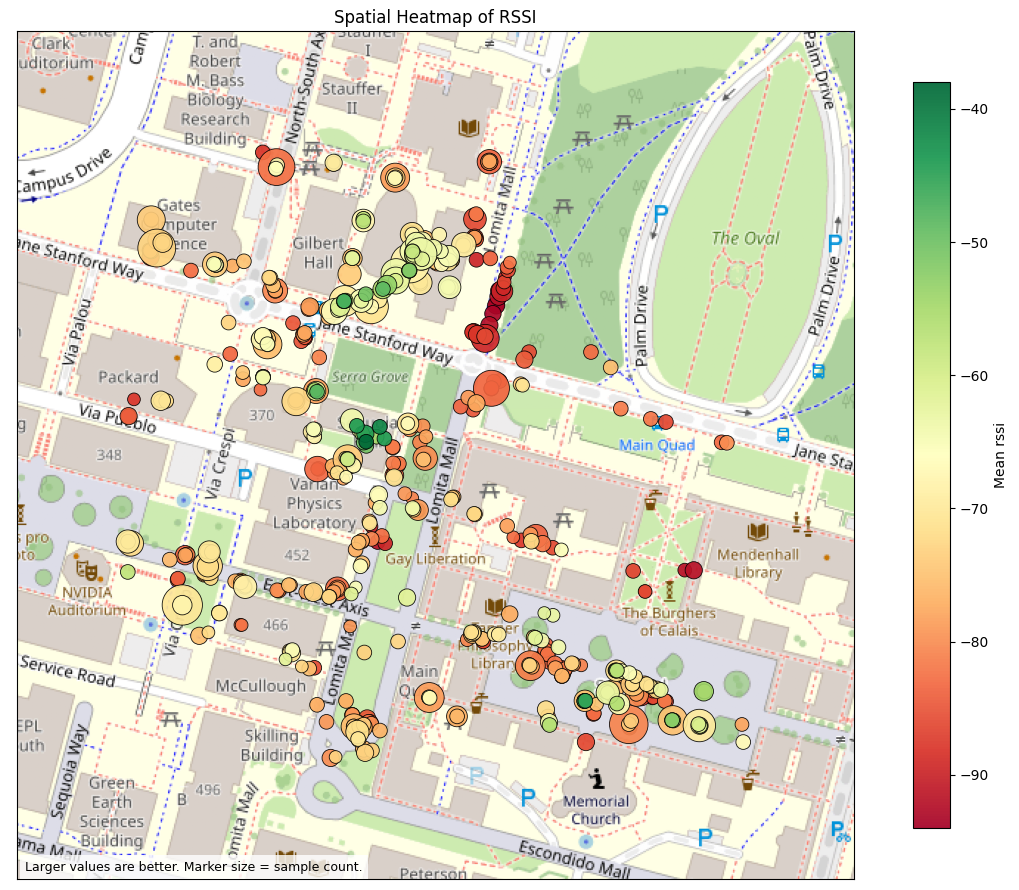
\includegraphics[width=0.38\textwidth]{rssi_heatmap.png}
%   \vspace{-60pt}
% \end{wrapfigure}

After cleaning, we reduced the raw data to a cleaned dataset with the following variables. We also decided to restrict our focus to the area surrounding Sequoia Hall, depicted in Figure \ref{fig:rssi-heatmap}, for which we have 3,869 samples at the time of writing.
\begin{enumerate}
    \item \texttt{date}, \texttt{time\_pdt}: temporal measurements
    \item \texttt{latitude}, \texttt{longitude}, \texttt{floor}: location and altitude measurements. The priority for the various location sources are to trust iPhone data over the CoreLocation data. 
    \item \texttt{indoor}: indicator for indoor vs. outdoor
    \item \texttt{signal\_measured}: indicator for whether sensor could receive signal
    \item \texttt{rssi}, \texttt{noise}: received signal strength indicator and signal noise
\end{enumerate}

\section{Exploratory Analysis}

% \begin{wrapfigure}{r}{0.4\textwidth}
%   \centering
%   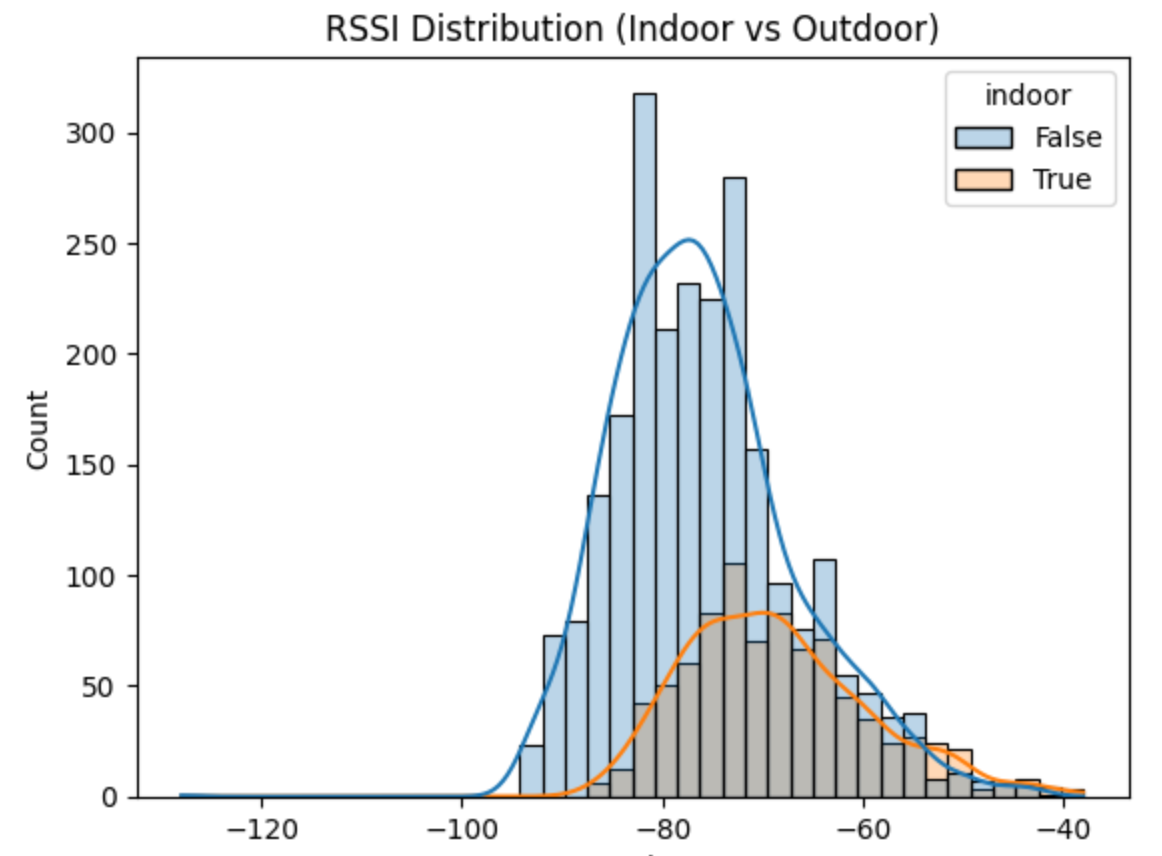
\includegraphics[width=0.38\textwidth]{indooroutdoor.png}
%   \vspace{-10pt}
% \end{wrapfigure}

Our primary target variable is \texttt{rssi} and to a lesser extent, \texttt{noise}. We observed that \texttt{rssi} has a much higher variance. The main predictors of interest are \texttt{latitude}, \texttt{longitude}, \texttt{indoor}, and \texttt{time\_pdt}.

To verify that \texttt{indoor} had more of an effect than could be captured by \texttt{latitude} and \texttt{longitude}, we examined the distribution of \texttt{rssi} conditioned on \texttt{indoor}. In Figure \ref{fig:indoor-outdoor}, we see that there is a clear distribution shift. This is something important to consider for our model.

Next, we checked to see whether the time of day, encoded in \texttt{time\_pdt}, had any meaningful effect on \texttt{rssi}. To do this, we fit a KNN of \texttt{rssi} on \texttt{latitude}, \texttt{longitude}, and \texttt{indoor}, using $5$-fold grid search cross validation. We then plotted the residuals against \texttt{time\_pdt} and observed that there was no meaningful relationship. The residuals appeared very homooskedastic and a linear regression yielded a slope of $-0.00026$. We observed a similar effect for the residuals of \texttt{noise} on \texttt{time\_pdt}. As such, we conclude that the difficulty of modeling \texttt{time\_pdt} significantly outweighs the its statistical importance.

% \begin{wrapfigure}{r}{0.4\textwidth}
%   \centering
%   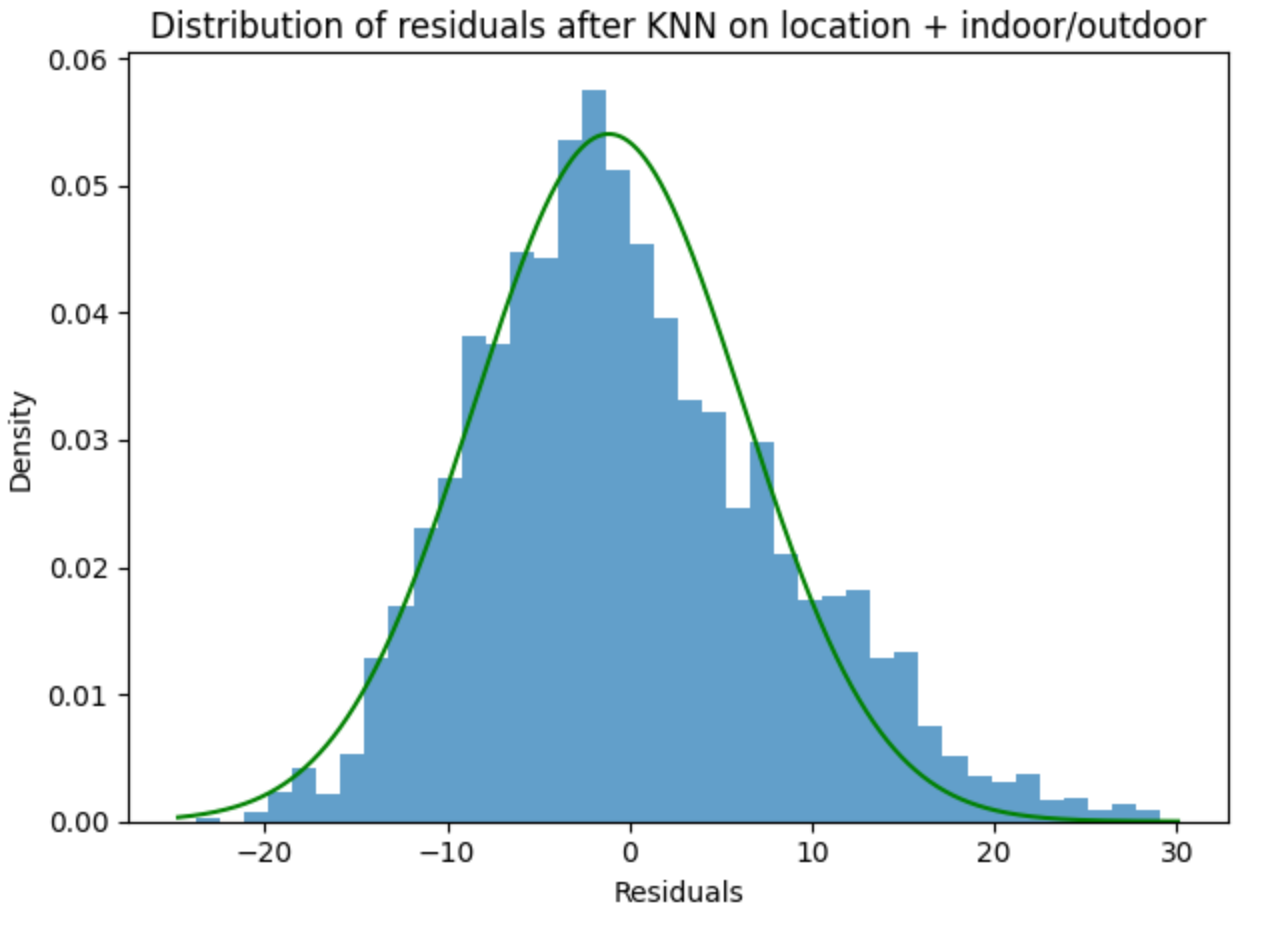
\includegraphics[width=0.38\textwidth]{error.png}
%   \vspace{-10pt}
% \end{wrapfigure}


Finally, to get some ideas about how to model our measurement error, we inspected the distribution of the residuals. This plot was quite sensitive to the KNN hyperparameters. For the optimal setting, we observed Figure \ref{fig:error}, which is overlayed with a rough Gaussian approximation. We see that the residuals are slightly right-skewed, but this effect was not always present when we ran this EDA pipeline at various stages of our data collection process. Also, when we chose smaller numbers of neighbors, the residuals became very symmetric, though they sharpened to more of a Laplace-like distribution than Gaussian. Overall, despite some mild skewness, the residuals are consistently unimodal and approximately symmetric under reasonable model settings, making a Gaussian error assumption a mathematically practical and sufficiently accurate approximation for subsequent modeling.

\section{Refined Model Sketch}

At a high level, we plan to model the latent WiFi strength field as a spatial Gaussian process. 

A literature search showed that there is extensive work in modeling RSSI \cite{ferris_gaussian_2006, kumar_gaussian_2016} as a Gaussian process, though for the end goal of device localization. These works learn a Gaussian process per WiFi access point, and use these to form a likelihood for the position of the device based on the known positions of the access points, and then estimate the device's position from this model. While we aren't interested in the same task, the main takeaways for us are that the access points dictate a lot of the structure in WiFi measurements. One simple approach would be to encode this in the covariance kernel. This is technically accessible to us, as \verb|wdutil| records a \verb|bssid| field corresponding to the ID of the access point. However, null observations naturally don't have a \verb|bssid| assigned.

For us, a preliminary model to serve as a baseline might take the following form.
\[
    \texttt{RSSI} \sim \GP(m, \K) + \epsilon
\]
where $m: \R^3 \to \R$ is a mean function that takes in \texttt{latitude}, \texttt{longitude}, and \texttt{indoors} (with some form of standardization), $\K: \R^3 \times \R^3 \to \R$ is a covariance kernel, and $\epsilon$ is measurement noise, which is assumed to be Gaussian as discussed above. The most salient challenge is how to handle the errors in our location measurements, which do not seem well-behaved based on our EDA.

For a more refined model, we can introduce modeling of the access points. A reasonable assumption is that there is an access point in each building, though we could treat their locations as an unknown parameter as well. We could either fit a $\GP$ for each access point, or encode distance from an access point as a fourth dimension in the global $\GP$ described above.

\newpage

\bibliographystyle{plain}
\bibliography{references}

\section*{AI Use Statement}

AI was used extensively to research the easiest way to collect data and was used to write the scripts and iOS shortcuts used for collection. It was also used to implement some of the data wrangling. 

\section*{GitHub Repository: \url{https://github.com/kevinzluo/where-my-wifi}}
\end{document}

 